\section {Чебурашка (Марковские цепи)}

Есть такой персонаж --- Чебурашка. Он же у нас --- некая система, которая может находиться в двух состояниях --- $a$ (хорошее настроение) и $b$(плохое настроение). Если мы находимся в состоянии $a$, вероятность перейти в состояние $b$ --- 0.7. Вероятность перейти из этого состояния обратно в состояние $a$, соответственно --- 0.3. Если мы находимся в состоянии $b$, вероятность перейти в состояние $a$ --- 0.6, вероятность перейти в состоянии $b$ ---  0.4.

\includegraphics[width=80mm]{ Cheburashka.png}

Допустим, он стартовал из состояния $a$. $S_t$ - состояние в момент времени $t$. 
Нас интересует вероятность того, что $S_t=a$. 
Особенно нас интересует предел при $t\to \infty$, то есть с какой вероятностью через много-много лет Чебурашка будет в хорошем настроении?
В матричном виде получается, что эта системка --- чистая линейная алгебра. Давайте мы введем вектор вероятностей:

$x_t = \left( \begin{array}{ll}
		P(S_t=a) & P(S_t=b) \\
		\end{array} \right).\\	$
Если Чебурашка стартует с хорошим настроением, то начальный вектор вероятностей:
$x_0= \left( \begin{array}{l}
		1 \\ 
		0\\
		\end{array} \right)\\  $
				
Найдем вектор вероятностей для следующего дня ($t=1$):
$P(S_1=a)=0.3\\
P(S_1=b)=0.7\\
x_1= \left( \begin{array}{l}
		0.3 \\ 
		0.7\\
		\end{array} \right)\\ $
Выпишем $x_2$, и все станет ясно:
$P(S_2=a)=0.3\cdot 0.3+0.7\cdot0.6\\
P(S_2=b)=0.3\cdot0.7+0.7\cdot0.7\\ $
Можем записать в общем виде:
$P(S_{t+1}=a)=P(S_t=a)\cdot0.3+P(S_t=b)\cdot0.6\\
P(S_{t+1}=b)=P(S_t=a)\cdot0.7+P(S_t=b)\cdot0.4\\ $
В чистом виде матричная алгебра, потому что 
$x_{t+1}= 
\left( \begin{array}{ll}
		0.3  0.7\\
		0.6  0.4\\
\end{array} \right)\cdot
x_t
\left( \begin{array}{l}
		S_t=a\\
		S_t=b\\
\end{array} \right)\\ $
$x_{t+1}$ находится в явном виде.
Матрица $\left( \begin{array}{ll}
		0.3  0.7\\
		0.6  0.4\\
\end{array} \right)$  ---  $P$. Тогда:
$x_1=Px_0\\
x_2=Px_1=P^2 x_0\\
x_3=Px_2=P^3x_0\\
x_n=P^nx_0\\ $

Возьмем и возведем матрицу в n-ую степень.
Матрица $P$ представима в виде:
$P = \left( \begin{array}{ll}
		0.3 & 0.6\\
		0.7 & 0.4\\
		\end{array} \right) =C \cdot D\cdot C^{-1}
$, где $C$ --- матрица из собственных векторов, $D$ --- матрица собственных значений
$\left( \begin{array}{ll}
		\lambda_1  & 0\\
		0  & \lambda_2\\
		\end{array} \right)\\ $
Найдем собственные числа:
			
$\begin{vmatrix}
	0.3-\lambda & 0.6\\
	0.7 & 0.4-\lambda
\end{vmatrix}=0\\
(0.3-\lambda)(0.4-\lambda)-0.6\cdot0.7=0\\
0.12-0.7\lambda+\lambda^2-0.42=0\\
\lambda^2-0.7\lambda-0.3=0\\
\lambda_1=1  \lambda_2=-0.3\\ $

Найдем собственные векторы:
$\left( \begin{array}{ll}
		-0.7 & 0.6\\
		0.7 & 0.6\\
		\end{array} \right) $
Подбираем любой собственный вектор:
  $h_1 = \left( \begin{array}{ll}
		6 & 7\\
		\end{array} \right)\\
\begin{pmatrix}
	0.6 & 0.6\\
	0.7 & 0.7
\end{pmatrix} \Rightarrow 
h_2=\left( \begin{array}{ll}
		1 & -1\\
		\end{array} \right) $
Получилось, что матрица P представима в виде:
$P=\left( \begin{array}{ll}
		6  & 1\\
		7  & -1\\
		\end{array} \right)
	\left( \begin{array}{ll}
		1  & 0\\
		0  & -0.3\\
		\end{array} \right)
	\left( \begin{array}{ll}
		6  & 1\\
		7  & -1\\
		\end{array} \right)^{-1}\\ $
В $P^n$ только серединка будет возводиться в степень.
В явном виде получили уравнение вероятности того, в каком настроении будет Чебурашка через $n$ дней: 
$		x_n=\left( \begin{array}{ll}
		6  & 1\\
		7  & -1\\
		\end{array} \right)
	\left( \begin{array}{ll}
		1  & 0\\
		0  & -0.3\\
		\end{array} \right)^n
	\left( \begin{array}{ll}
		6  & 1\\
		7  & -1\\
		\end{array} \right)^{-1} \cdot x_0 $
Найдем теперь предел $x_n$ при $n\to \infty$.
Если матрицу возвести в очень большую степень, то 1 останется 1, а -0.3 --- 0: 
$\lim_{n\to\infty}x_n=
	\left( \begin{array}{ll}
		6  & 1\\
		7  & -1\\
		\end{array} \right)
	\left( \begin{array}{ll}
		1  & 0\\
		0  & 0\\
		\end{array} \right)
	\left( \begin{array}{ll}
		6  & 1\\
		7  & -1\\
		\end{array} \right)^{-1}\\ $
Можно руками досчитать уравнение:
$\lim_{n\to\infty}x_n=
	\left( \begin{array}{ll}
		6  & 0\\
		7  & 0\\
		\end{array} \right)
	\left( \begin{array}{ll}
		6  & 1\\
		7  & -1\\
		\end{array} \right)^{-1}\cdot x_0 $
		
$\lim_{n\to\infty}x_n=
	\left( \begin{array}{ll}
		6  & 0\\
		7  & 0\\
		\end{array} \right)\cdot 1/13\cdot
	\left( \begin{array}{ll}
		1  & -1\\
		-7  & 6\\
		\end{array} \right)\cdot x_0 $

$\lim_{n\to\infty}x_n=
	(-1/13)\cdot 
	\left( \begin{array}{ll}
		6x_1  & 6x_2\\
		7x_1  & 7x_2
		\end{array} \right)=
	\left( \begin{array}{l}
		6/13\\
		7/13\\
		\end{array} \right) $
		
Получили, что ответ не зависит от $x_0$: еважно, как мы начинали --- вероятности состояний $a$ и $b$ в пределе будут одинаковы. Этот результат можно было получить и проще.

Представим старого Чебурашку через много-много лет. Наступает следующий день, и бесконечно старый Чебурашка мало чем отличается от бесконечно старого Чебурашки, прожившего еще один день.
Математически: есть вектор $x_{\infty}$. Если пройдет еще один день, то он не должен измениться. 
У нас есть зависимость:
$x_{t+1}=Px_t$
Если мы возьмем предел слева и справа от зависимости $x_t$ и $x_{t+1}$(предположив, что предел есть), получим: $\lim_{t\to\infty}x_\infty=Px_{\infty}$ 
Сумма вероятностей равна 1, и получается простенькое уравнение ($r$ --- вероятность состояния $a$):
$\left( \begin{array}{l}
		r\\
		1-r
		\end{array} \right)=
 \left( \begin{array}{ll}
		0.3  & 0.6\\
		0.7  & 0.4
		\end{array} \right)
\left( \begin{array}{l}
		r\\
		1-r
		\end{array} \right) 
x_\infty=lim_{t\to\infty}x_t=
\left( \begin{array}{l}
		r\\
		1-r\\
		\end{array} \right) 
r=0.3r+0.6(1-r) \Rightarrow r=6/13 $
		
Получили те же 6/13, только просто.
Ремарка: Предполагалось, что предел существует, из-за свойств матрицы $P$(его собственные значения меньше либо равны 1,это потом отдельно как-нибудь докажем) это действительно так
Давайте пойдем дальше. Как применить к игре Паррондо Чебурашку?


Теорию марковских цепей отложим на следующий раз. Сейчас --- игра паррондо
У нас была игра Б. Возможно 3 остатка от деления на 3 --- 0, 1 и 2. Давайте чертить 
стрелочки. Тут все красиво: здесь --- по часовой стрелке, тут --- против.
Если сейчас остаток от деления на 0, какова вероятность что следующий остаток будет 1?
Сейчас остаток 0 - сумма в кошельке делится на 3. С вероятностью 0.05 я получу 1 рубль,
и остаток станет 1, с вероятностью 0.95 он станет 2. Сейчас оствток --- 2: нужно прибавить рубль --- 0.7, рубль --- 0.3. Аналогично для рубля. Не будем матрицу составлять. 
У нас много случайных величин, мы пока последим за $X_n$ --- остатком от деления на 3 суммы в кошельке в момент времени $n$. 
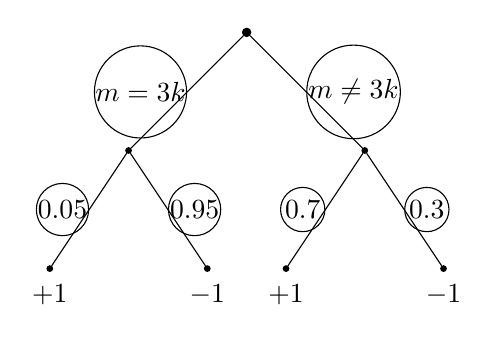
\begin{tikzpicture}[grow=down]
 \tikzset{edge from parent/.style=
     {draw, edge from parent path={(\tikzparentnode) -- (\tikzchildnode)}}}
\tikzstyle{mystart} = [circle, minimum width=3pt,fill, inner sep=0pt]
\tikzstyle{mydot} = [circle, minimum width=2pt,fill, inner sep=0pt]
\tikzstyle{level 1}=[sibling distance=3cm]
\tikzstyle{level 2}=[sibling distance=2cm]
	\node[mystart] {} 
	child { node[mydot] {}
		child { node[mydot, label=below: $+1$] {}
		edge from parent node[left] {$0.05$} }
		child { node[mydot, label=below: $-1$] {}
		edge from parent node[right] {$0.95$} }
	edge from parent node[left] {$m=3k$} }
	child { node[mydot] {}
		child { node[mydot, label=below: $+1$] {}
		edge from parent node[left] {$0.7$} }
		child { node[mydot, label=below: $-1$] {}
		edge from parent node[right] {$0.3$} }
	edge from parent node[right] {$m\ne3k$} };
\end{tikzpicture}

\begin{tikzpicture}[->,>=stealth',shorten >=1pt,auto,node distance=3.5cm,
  thin,main node/.style={circle, draw, minimum width=16pt, inner sep=0.5pt}]
\node[main node] (1) {$0$};
\node[main node] (2) [below left of=1] {$1$};
\node[main node] (3) [below right of=1] {$2$};
\path
(1) edge[bend right] node[left] {0.05} (2)	
(2) edge[bend right] node[below] {0.7} (3)	
(3) edge[bend right] node[right] {0.7} (1)	
(1)	edge[left] node[left]  {0.35} (3)	
(2)	edge[left] node[right] {0.3} (1)
(3) edge[left] node[above] {0.3} (2);	
\end{tikzpicture}

$X_t$ --- суммы в кошельке в момент времени $t$
$\lim{n\to\infty}(X_n=0)
 \lim{n\to\infty}(X_n=1)
 \lim{n\to\infty}(X_n=2) $
 Посчитаем пределы. Как мы это будем делать? Введем вектор вероятностей $y_n$:

 $y_n=\left( \begin{array}{l}
		P(X_n=0)\\
		P(X_n=1)\\
		P(X_n=2)
		\end{array} \right) $
Как и в случае с Чебурашкой, $y_{n+1}=P\cdot y_n\\ $. Только размерность матрицы P будет другая. Найдем матрицу P в этом случае. 
Какова вероятность перейти в состояние 0, если я был в состоянии 0 - 0: нули по диагонали.
Если я был в состоянии 0, то какова вероятность перейти в состояние 

$\left( \begin{array}{l}
		P(X_{n+1}=0)\\
		P(X_{n+1}=1)\\
		P(X_{n+2}=2)
		\end{array} \right)=
\left( \begin{array}{l}
		0\cdot P(X_n=0)+0.3P(X_n=1)+0.7P(X_n=2)\\
		0.05P(X_n=0)+0\cdot P(X_n=1)+0.3P(X_n=2)\\
		0/05P(X_n=0)+0.7P(X_n=1)+0\cdot P(X_n=2)\\
		\end{array} \right) $
Значит, наша матрица P имеет следующий вид:
$P=\left( \begin{array}{lll}
		0    &0.3 & 0.7\\
		0.05 &0 & 0.3\\
		0.05 &0.7 & 0\\
		\end{array} \right) $
И мы хотим найти $y_\infty=\liminf{y_n}$, то есть если я буду долго-долго играть в эту игру, каковы будут вероятности иметь остатки 0,1 и 2 от деления на 3 суммы в кошельке. Не будем сейчас считать собственные числа. Пойдем по идее $y_\infty=P\cdot y_\infty$
Введем две неизвестных(a - вероятность 0, b- вероятность 1): 

$\left( \begin{array}{l}
		a\\
		b\\
		1-a-b
		\end{array} \right)=
\left( \begin{array}{l}
		0+0.3b+0.7(1-a-b)\\
		0.05a+0+0.3(1-a-b)\\
		0.05a+0.7b+0\\
		\end{array} \right) $
Двух уравнений для двух неизвестных достаточно, поэтому третье не будем дальше смотреть.
Решаем:

$\begin{cases}
a  =  0.3b+0.7-0.7a-0.7b \\
b  =  0.05a+0.3-0.3a-0.3b 
\end{cases}
$

$\begin{cases}
1.7a + 0.4b  =  0.7 \\
0.25a + 1.3b  =  0.3 
\end{cases}$




Домножим все на 10, и тогда получается:
$a=\frac{\begin{vmatrix}
	7 & 4\\
	3 & 13
\end{vmatrix}}
{\begin{vmatrix}
	17 & 4\\
	2.5 & 13
\end{vmatrix}}=\frac{91-12}{221-10}=\frac{79}{211}\\ $

Нашли $a$, точно так же находим $b$:
$b=\frac{\begin{vmatrix}
	17 & 2.5\\
	7 & 3
\end{vmatrix}}
{211}=\frac{33,5}{211}\\ $

Это нам дает возможность оперделить,выигрышная эта игра или проигрышная, потому что мы знаем, что когда пройдет много-много времени, с вероятнотсью 79/211 остаток будет кратен 0. 
Я знаю:
$\frac{79}{211} \Rightarrow m=3k\\
\frac{132}{211} \Rightarrow m\ne 3k\\ $
Посмотрим мат.ожидание выигрыша через много-много лет:
$\frac{79}{211}(0.05-0.95)+\frac{132}{211}(0.7-0.3)=-0.9\frac{79}{211}+\frac{132}{211}0.4=\frac{132\cdot 4-79\cdot9}{10\cdot211}<0$
То есть сама по себе эта игра через много времени будет приносить отрицательное матожидание выигрыша. А что будет, если ее комбинировать с игрой А? Не будем до конца доводить вычисления, просто идейно:
%игра А-в дерево
%дерево общее
Можем дерево упростить: сначала смотреть, делится ли сумма в кошельке на 3, и уже затем с вероятностью 1/2 выбирать игру А или игру В. Тогда получается вот такое дерево:
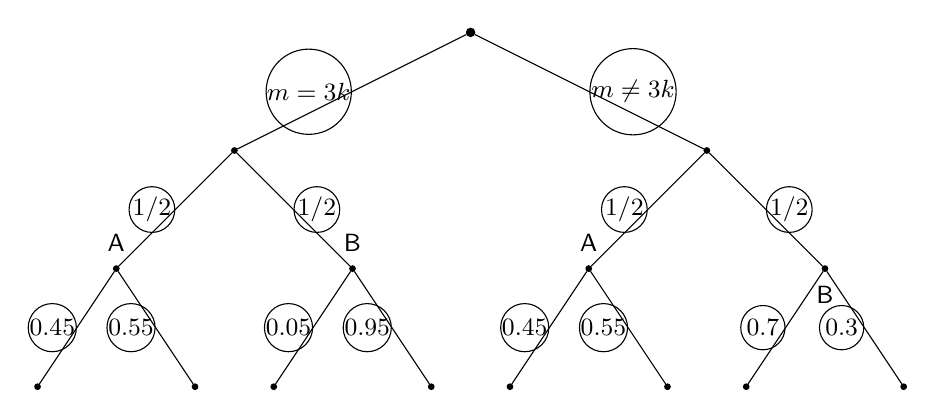
\begin{tikzpicture}[grow=down]
 \tikzset{edge from parent/.style=
     {draw, edge from parent path={(\tikzparentnode) -- (\tikzchildnode)}}}
\tikzstyle{mystart} = [circle, minimum width=3pt,fill, inner sep=0pt]
\tikzstyle{mydot} = [circle, minimum width=2pt,fill, inner sep=0pt]
\tikzstyle{level 1}=[sibling distance=6cm,font=\sffamily\small]
\tikzstyle{level 2}=[sibling distance=3cm,font=\sffamily\small]
\tikzstyle{level 3}=[sibling distance=2cm,font=\sffamily\small]
	\node[mystart] {} 
	child { node[mydot] {}
		child { node[mydot, label=above:A] {}
			child { node[mydot] {}
			edge from parent node[left] {${\tiny 0.45}$} }
			child { node[mydot] {}
			edge from parent node[left] {$\small 0.55$} }
		edge from parent node[left] {$1/2$} }
		child { node[mydot, label=above: B] {}
			child { node[mydot] {}
			edge from parent node[left] {$0.05$} }
			child { node[mydot] {}
			edge from parent node[left] {$0.95$} }
		edge from parent node[right] {$1/2$} }
	edge from parent node[left] {$m=3k$} }
	child { node[mydot] {}
		child { node[mydot,label=above:A] {}
			child { node[mydot] {}
			edge from parent node[left] {$0.45$} }
			child { node[mydot] {}
			edge from parent node[left] {$0.55$} }
		edge from parent node[left] {$1/2$} }
		child { node[mydot, label=below:B] {}
			child { node[mydot] {}
			edge from parent node[left] {$0.7$} }
			child { node[mydot] {}
			edge from parent node[left] {$0.3$} }
		edge from parent node[right] {$1/2$} }
	edge from parent node[right] {$m \ne 3k$} };
\end{tikzpicture}
 Получается, что мы можем усреднить эти вероятности и получить, что игра 
  $1/2A+1/2B$ эквивалента следующей игре:



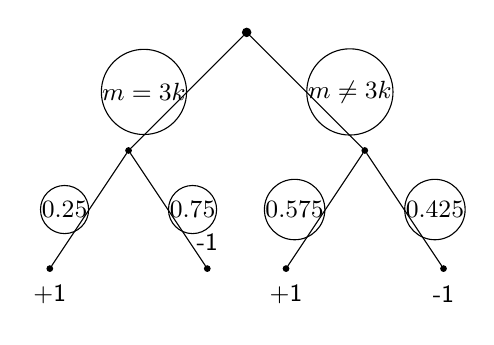
\begin{tikzpicture}[grow=down]
 \tikzset{edge from parent/.style=
     {draw, edge from parent path={(\tikzparentnode) -- (\tikzchildnode)}}}
\tikzstyle{mystart} = [circle, minimum width=3pt,fill, inner sep=0pt]
\tikzstyle{mydot} = [circle, minimum width=2pt,fill, inner sep=0pt]
\tikzstyle{level 1}=[sibling distance=3cm,font=\sffamily\small]
\tikzstyle{level 2}=[sibling distance=2cm,font=\sffamily\small]
	\node[mystart] {} 
	child { node[mydot] {}
		child { node[mydot, label=below:+1] {}
		edge from parent node[left] {$0.25$} }
		child { node[mydot, label=above: -1] {}
		edge from parent node[right] {$0.75$} }
	edge from parent node[left] {$m=3k$} }
	child { node[mydot] {}
		child { node[mydot,label=below:+1] {}
		edge from parent node[left] {$0.575$} }
		child { node[mydot, label=below:-1] {}
		edge from parent node[right] {$0.425$} }
	edge from parent node[right] {$m\ne 3k$} };
\end{tikzpicture}

Для такой игры мы можем с помощью цепей Маркова посчитать предельные вероятноти остатка 0, остатка 1, остатка 2. Зная предельные вероятности, узнаю средний выигрыш. Получится, что он все-таки получается  положительный.
Вот такое чудо: играешь долго-долго в игру А, она отрицательный выирыш дает, Б - тоже, а с вероятностями --- положительный выигрыш.
Заодно мы и цепи Маркова прошли, хотя бы на практике. Осталось дома что-нибудбь порешать.



Упражнение 1.
Мышь бегает по коридорчикам:

\begin{tikzpicture}[->,>=stealth',shorten >=1pt,auto,node distance=3cm,
  thin,main node/.style={circle, draw, minimum width=16pt, inner sep=0pt}]
\node[main node] (1) {a};
\node[main node] (2) [below left of=1] {b};
\node[main node] (3) [below right of=1] {c};
\path[every node/.style={font=\sffamily\small}]
 (1) edge[loop above] node {0.1} (1)
 	 edge [bend right] node {0.9} (2)
 (2) edge[loop left] node {0.2} (2)
 	 edge [bend right] node {0.8} (3)
 (3) edge [loop right] node{0.3} (3)
 	 edge [bend right] node {0.7} (1);
\end{tikzpicture}

Нужно найти:
$\P(S_t=a)$, $\P(S_t=b)$, $\P(S_t=c)$ при $t\to\infty$

Упражнение 2. Даша и Глаша. 
Даша и Глаша подкидывают <<правильную>> монетку до тех пор, пока не выпадет ОРО или РРР. Глаша выигрывает в случае РРР, Даша ---  в случае ОРО. 
Найти вероятность того, что выиграет Даша.


Упражнение 3.
Изначально конь стоит на А1 и дальше ходит равновероятно любым возможным способом. 
Какой процент своей бесконечной жизни конь проведет в стойле $H8$?


\section{Байесовские сети}

В теории вероятностей о причинно-следственных связях не говорят: есть совместная функция плотности $X$ и $Y$, а кто причина, кто следствие, не говорят: $X$ может влиять на $Y$, $Y$ может влиять на $X$ или какая-то $Z$ может влиять и на $X$, и на $Y$.  
Одна и та же формула и в случае зависимого $Y$, и в случае зависимого $X$: $p(x)\cdot p(y\mid x)=p(x\mid y)=p(y)\cdot p(x\mid y)$. Но когда $X$ влияет на $Y$, логичнее запись $p(x)\cdot p(y\mid x)$.

По такой логике можно расклаывать на сомножители совместные функции плотности:
 для 
 
\begin{tikzpicture}[grow=right]
\tikzstyle{mycircle} = [circle, draw, minimum width=16pt, inner sep=0pt] % node style
\tikzset{edge from parent/.style=
     {-angle 45, % рисуем стрелочку
     % это магическое заклинание направляющее ребра к центру узла, а не к точке под узлом:
     draw, edge from parent path={(\tikzparentnode) -- (\tikzchildnode)}}}
\tikzstyle{every node}=[mycircle]
\node {$X$} % создаем узел 
    child { node {$Y$} } ;
\end{tikzpicture}

$p(x,y)=p(x)p(y \mid x)$

для

\begin{tikzpicture}[grow=right]
\tikzstyle{mycircle} = [circle, draw, minimum width=16pt, inner sep=0pt] % node style
\tikzset{edge from parent/.style=
     {-angle 45, % рисуем стрелочку
     % это магическое заклинание направляющее ребра к центру узла, а не к точке под узлом:
     draw, edge from parent path={(\tikzparentnode) -- (\tikzchildnode)}}}
\tikzstyle{every node}=[mycircle]
\node {$X$} % создаем узел 
    child { node {$Y$}} 
    child {node {$Z$}} ;
\end{tikzpicture} 


$p(x,y,z)=p(x)\cdot p(y \mid x) p(z \mid x)$

для

\begin{tikzpicture}[->,>=stealth',shorten >=1pt,auto,node distance=1.5cm,
  thin,main node/.style={circle, draw, minimum width=16pt, inner sep=0pt}]
\node[main node]  (1) {$X_1$}; 
\node[main node] [below right of=1] (2) {$X_2$}; 
\node[main node] [below left of=1] (3){$X_3$} ;
\path
(1) edge node [right] {} (3)
	edge node [left] {} (2)
(2) edge node [left] {} (3);
\end{tikzpicture}


$p(X_1,X_2,X_3)=p(X_1)p(X_2\mid X_1) p(X_3 \mid X_1,X_2)$

для

\begin{tikzpicture}[->,>=stealth',shorten >=1pt,auto,node distance=1.7cm,
  thin,main node/.style={circle, draw, minimum width=16pt, inner sep=0pt}]
\node[main node] (1) {$X_1$};
\node[main node] (2) [below of=1] {$X_2$};
\node[main node] (3) [below of=2] {$X_3$};
\node[main node] (4) [left of=2]{$X_4$};
\path
(1) edge node {} (2)
(2) edge node {} (3)
(4) edge node {} (3);
\end{tikzpicture}


$p(x_1,X_2,X_3,X_4)=p(X_1)p(X_4)p(X_2\mid X_1)p(X_3\mid X_1,X_4)$

Мысль такая: нужно всегда  перемножать условные вероятности иксов при фиксированном родителе.



Проведем байесовский анализ для простейших случаев.
Модель 1. Есть случайные величины $X_1$,$X_2$,...
Они независимы и имеют следующее распределение:

$\begin{array}{c|ccc}
    {} &  1  & 2  & 7   \\
\hline
    {p} &  {\beta} & {2\beta} & {1-3\beta}   \\
\end{array}$

Есть классические методы: можем оценивать бета с помощью метода максимального правдоподобия или моментов. 
Пусть выборка: $X_1=1$, $X_2=2$, $X_3=2$, $X_4=7$.
Можем оценить  $\beta$ с помощью метода моментов, метода максимального правдоподобия и байесовского метода.


Что говорит метод моментов? 
Если число наблюдений велико, то среднее по выборке должно примерно равняться мат. ожиданию:
 $\E(X_i)=\beta+4\beta+7-21\beta=16\beta$. 
Тогда по методу моментов: $\bar{X}=7-16\hat{\beta}\\
\hat{\beta}_{mm}=(7-\bar{X})/16=1/4$

Что говорит метод максимального правдоподобия?
Надо максимизировать по $\beta$ $\P(X_1=1 \cap X_2=2 \cap X_3=2 \cap X_4=7)$
Получается: $4\beta^3(1-3\beta) \Rightarrow \max_{\beta}$
Считаем, что то, что нам попалось --- самые часто встречающиеся наблюдения.
Решаем задачу максимизации с позиции девятиклассника: $4\beta \cdot \beta \cdot \beta \cdot \alpha$
 Если числа не равны, то я возьму от большего кусочек и передам в другой. Тогда сумма не поменяется (сумма вероятностей равна 1). Получается, что все они равны. $\beta=1/4$ (совпали оценки случайно)

Байесовский подход.
До получения данных должно быть представление о $\beta$. Нарисуем байесовскую сеть: 

\begin{tikzpicture} [grow=down]
\tikzstyle{mycircle} = [circle, draw, minimum width=16pt, inner sep=0pt] % node style
\tikzset{edge from parent/.style=
     {-angle 45, % рисуем стрелочку
     % это магическое заклинание направляющее ребра к центру узла, а не к точке под узлом:
     draw, edge from parent path={(\tikzparentnode) -- (\tikzchildnode)}}}


\tikzstyle{every node}=[mycircle]
\node {$\beta$} % создаем узел 
    child { node {$X_1$}} 
    child {node {$X_2$}}
    child {node {$X_3$}}
    child {node {$X_4$}} ;
\end{tikzpicture} 

Пишем совместную функцию плотности: $p(X_1,X_2,X_3,X_4,\beta)=p(\beta)p(X_1 \mid \beta)p(X_2 \mid \beta)p(X_3 \mid \beta)p(X_4 \mid \beta)$

Априорное мнение о  $\beta: p(\beta)$.
Порассуждаем:$\beta \in [0;1/3]$
Будем для простоты верить, что  $\beta$ распределено равномерно на этом промежутке. 
Мы вложились в мнение о $\beta$: мы получим наше мнение о $\beta$ с учетом вероятности $p(\beta \mid X_1,X_2,X_3,X_4)=\frac{p(\beta,X_1,X_2,X_3,X_4)}{p(X_1,X_2,X_3,X_4}\sim p(\beta)p(X_1 \mid \beta)p(X_2 \mid \beta)p(X_3 \mid \beta)p(X_4 \mid \beta)=3\beta^2\beta(1-3\beta)=\beta^3(1-3\beta)$

Интеграл под функцией плотности должен быть равен 1, значит мы можем вычислить константу:
$\int_0^{1/3} \beta^3(1-3\beta)dt=\frac{(1/3)^4}{4}-\frac{3(1/3)^5}{5}=\frac{1}{81\cdot20}$
Значит, с учетом имеющихся наблюдений функция плотности:
$81\cdot20\cdot\beta^3(1-3\beta)$
Таков Байесовский подход: положите свое мнение на входе о параметре, и на выходе получите это мнение с учетом результатов наблюдений. 
При этом Байесовский подход дает нам оценку целой функции плотности, а как точечную оценку мы можем выбрать моду, матожидание, среднее. Можем построить интервал, в который $\beta$ войдет с вероятностью, допустим, 90\%.

Почему Байесовский метод дает нам распределение $\beta$, хотя это число?
Мягкий подход: функция плотности выражает всю неуверенность о $\beta$
Жесткий подход: почему $\beta$ вообще должно быть числом? Допустим, $\beta$ - это рост слона: в детстве он голодал, он рос, его рост  к сегодняшнему числу --- случайная величина: его могли не кормить и.т.д. Рост --- результат случайных событий и сам является случайной величиной.

Мы можем смотреть, насколько устойчив результат при разных верах --- насколько будет устойчиво условное распределение при разных априорных распределениях. Если при разных верах условное распределение несильно меняется, это хорошо --- значит, мы взяли достаточное количество наблюдений. 









